%% josis.tex 1.2   2009-06-11    JoSIS latex template
%------------------------------------------------------------------
% Filename: josis.tex
%
% This file is intended as a template for typesetting articles for the
%
%                        Journal of Spatial Information Science.
%
% Please edit this template to generate your own formatted manuscripts
% for submission to JOSIS. See http://josis.org for further details.
%
% The template was developed by Matt Duckham (http://www.duckham.org)
%

% Required documentclass definition for JOSIS
\documentclass{josis}
\usepackage{graphics}
\usepackage{subfigure}
\usepackage[colorlinks=true,urlcolor=blue]{hyperref}
\usepackage{enumerate}

% Link as footnote
\newcommand{\furl}[1]{$\,$\footnote{$\,$\url{#1}}}

% Article details for accepted manuscripts will be added by editorial staff
%\josisdetails{%
%   volume=0, number=0, year=2009, firstpage=0, lastpage=1,
%   received={January 1, 2009},
%   revised={March 1, 2009},
%   accepted={May 1, 2009},
%   published={June 1, 2009}
%}


% Add the running author and running title information
\runningauthor{\begin{minipage}{.9\textwidth}\centering Michel, Grizonnet, Jaen, Hermitte, Guinet, Harasse, Malik, Savinaud\end{minipage}}
\runningtitle{Large-scale segmentation of VHR satellite images using Orfeo ToolBox}

% Document begins
\begin{document}

% Insert your own title
\title{Large-scale segmentation of Very High Resolution satellite images using Orfeo ToolBox}

% Insert your manuscipts authors, affiliations, and addresses
\author{Julien Michel}
\author{Manuel Grizonnet}\affil{CNES, DCT/SI/AP, BPI 1219 18, avenue Edouard Belin, 31401 Toulouse Cedex 09 - France}
\author{Arnaud Jaen}
\author{Luc Hermitte}
\author{Jonathan Guinet}
\author{S\'ebastien Harasse}
\author{Julien Malik}
\author{Micka\"el Savinaud}
\author{Guillaume Pasero}\affil{CS Syst\`emes d'Information, Division ESPACE \& Renseignement - D\'epartement APPLICATIONS, Parc de la Grande Plaine - 5, Rue Brindejonc des Moulinais - BP 15872, 31506 Toulouse Cedex 05 - FRANCE}


\maketitle

% Add 5-10 keywords for every submission
\keywords{Open source software, segmentation, remote sensing images, GIS}

% Add a short abstract of 150-250 words
\begin{abstract}
Many high level techniques to analyze very high resolution remote
sensing images consider segmentation as a pre-processing
step. However, segmenting this kind of data is challenging: there are
of course issues such as the ability of the segmentation to fit the
objects of interest with high inner variance implied by the image
resolution, or the stability of the segmentation quality across large
or multiple scenes. This work tries to address yet another issue,
which is the segmentation algorithms scalability to process full very
high resolution remote sensing images. This latter issue prevent from
any assessment of a range of techniques at full scene scale.

In order to work around this issue, we reviewed data structures and
segmentation algorithms so as to design and implement into the Orfeo
ToolBox open source remote sensing library a generic framework for
the segmentation of very large images, which has been successfully
applied to Pleiades images and produces GIS-compatible outputs.

\end{abstract}


% Your main text begins here.
\section{Introduction}

With the increase of the spatial resolution of satellite images,
analysis techniques such as Object Based Image Analysis
(OBIA)~\cite{michel2010lazy} or Spatial
Reasoning~\cite{inglada2009qualitative,vanegas2009fuzzy,vanegas2010detection}
have become widely studied and used. Because they use objects rather
than pixels as their primitives, these methods are very well adapted
to represent and extract the information contained in very high
resolution imagery (VHR). Moreover, reasoning on objects is often
supported by very sound theories. Yet one of their severe weakness is
the process of obtaining the objects themselves: segmentation is
widely used as a pre-processing step for these techniques, and it is
well known that the task of segmenting all categories of object of
interest, across a large very high resolution scene and with a
controlled quality is a difficult task for which no method has reached
a sufficient level of performance to be considered as operational.

Even if we leave aside the question of segmentation quality and
consider that we have a method performing reasonably well on our data
and objects of interest, the task of scaling up segmentation to real
very high resolution data is itself challenging.  For instance a basic
Pleiades image~\cite{tinel2012orfeo} has an extent of 40 000 by 40 000
pixels, which corresponds to a memory size of 12.8 GB assuming a
4-bands image with 16 bits per pixel. First, we can not load the
whole data into memory, and there is a need for on the flow processing
which does not cope well with traditional segmentation
algorithms~\cite{shi2000normalized}. Second, the result of the
segmentation process itself is difficult to represent and manipulate
efficiently.

There are, to our best knowledge, few open source software able to
overcome these issues. In the frame of the development of the Orfeo
ToolBox\furl{www.orfeo-toolbox.org}, we therefore initiated some work
to provide software components for this purpose. The remaining of the
paper is organized as follows. Section~\ref{sec:otb} briefly
introduces the Orfeo ToolBox software, while section~\ref{sec:seg}
presents the large scale segmentation framework which is the main
focus of the paper.

\section{About the Orfeo ToolBox}\label{sec:otb}

The Orfeo Toolbox (OTB) is an open source (CeCILL license, similar to GPL), remote
sensing-oriented, image processing library~\cite{inglada2009orfeo}. It
has been initiated by the French Space Agency (CNES) in the frame of
the ORFEO accompaniment program~\cite{tinel2012orfeo}. Based on the
medical image processing library Insight ToolKit (ITK), OTB
provides to its users an extensive set of algorithms and
functionalities dedicated to remote sensing data exploitation. More
specifically, it embeds approaches to handle large data using
advanced streaming and multi-threading strategies. Thus, OTB-based
processing chains take advantages of both optimized Input/Output
access and streamed/multi-threaded filtering to perform efficient
processing.

OTB is based on a large set of open source libraries which contribute
to expand the OTB ecosystem. The main part of this ecosystem is
described in the figure~\ref{fig:ecosystem}. Through the use of these
libraries, it offers the possibility to manipulate and process the
main remote sensing data from optical to hyperspectral through SAR
sensors. The processing capabilities of OTB library covers a large set
of uses cases from optical calibration and data projection to image
segmentation and classification. An exhaustive list can be found in
the documentation.

\begin{figure}[!htb]
\centering
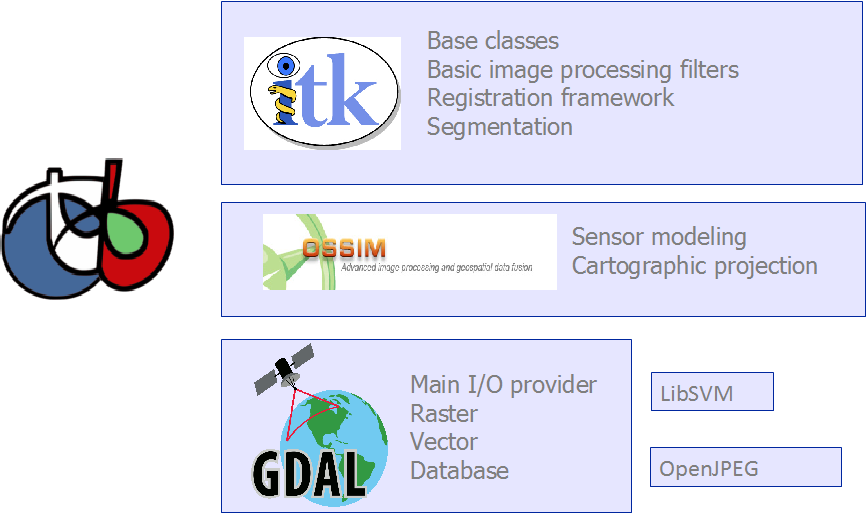
\includegraphics[width=0.8\textwidth]{Pictures/otb_ecosystem}\label{fig:ecosystem}
\caption{Orfeo ToolBox ecosystem}
\end{figure}

One of the main way to access to the OTB capabilities for end-users is
to use the set of applications offered by OTB (the other being to use
the C++ API directly). These applications have recently been
improved to answer to the increasing need to interface OTB
capabilities into other software and to provide a better access to
end-users. They are also designed as a plugin based architecture which allows auto-load into
appropriate tools without recompiling. Currently
Orfeo ToolBox ships the following tools:
\begin{itemize}
\item A command-line launcher,
\item A graphical launcher based on a Qt interface which provide
  ergonomic parameters setting, display of documentation, and progress
  reporting,
\item A SWIG interface, which allows to use any application into a
  high-level language such as Python or Java for instance.
\end{itemize}
Moreover, through the Sextante project, OTB applications are also
available into the QGIS software. QGIS users have therefore an easy
way to combine these processings with other tools.

As an open source project, OTB exposes its source code via a public
official repository. Moreover, the library is built and tested on a
nightly basis. The results are available publicly which ensures
multi-platform consistency and continuous validation. Last, OTB
encourages full access to the details of all the algorithms through
extensive documentation. This documentation is divided between class
documentations, the software guide~\cite{otbSoftwareGuide} which gives
some technical remote sensing processing background along with code
examples and a cookbook~\cite{otbCookBook} dedicated to non-developers.

\section{Segmenting very large images with Orfeo ToolBox}\label{sec:seg}


\subsection{Representations and data structures for segmentation results}

In this section, we review three standard structures to store
segmentation results, and explain why we selected the third one for
our framework.

The most common way of representing segmentation results from an image
processing perspective is to derive a raster where each pixel contains
the unique label of the segment it belongs to. Such a raster is also
known as label image. Yet this representation has numerous
drawbacks. First, accessing all pixels of a given segment identified
by its label requires parsing the whole label image. Second, storing
large segmentation results with billions of segments might require a
high number of bits to represent the label, thus increasing
dramatically the size of the output. Last, the constraint of label
uniqueness is very strong, yet not very useful: it is required since
label images only provides an implicit description of segments, based
on neighboring pixels with same labels. As a consequence, this representation is of
limited interest for our purpose.

A second representation of segmented image which is further from image
processing is the map of label objects~\cite{lehmann2008label}. A segment is
represented in Run Length Encoding (RLE), and all segments are indexed by a
unique label in a map. The RLE representation is more compact, the map allows
fast access to a segment given its label, and it also allows to store attributes
related to a segment, which is a first step toward Object Based Image
Analysis. The main drawback of this representation is that there are no standard
file format able to store it on a file system, and it requires to convert either
to or from raster or vector representation at each read or write
operation. Moreover, this representation is neither really raster nor really
vector. Therefore, operations like scanning pixels segment or following its
contour are more complex.

Neither of these two structures can fit our needs: the first one is
highly inefficient, while the second one lacks of existing file
formats. We chose to store our segmentation results as boundaries in a
vector structure and file format. This has numerous advantages. First,
it overcomes the issue of scaling up to large image segmentation: a
collection of vector objects, i.e. polygons or multi-polygons, is a
compact representation which will grow linearly with the size of the
image, and does not need an explicit unique indexing label. Second,
there are several file formats and even databases to represent this
kind of vector data, especially in the GIS world. Last, using such
formats guarantees a full interoperability between the segmentation
tools and most GIS software.

As described in the next section, we intend to derive a generic framework for
large scale remote sensing images segmentation, thus we need to be compatible
with the raster output of most segmentation algorithms, which usually produce a
label image. For this purpose, we need a component for exact conversion between
the raster and the vector representation. We take advantage of the
polygonization and rasterization algorithms provided by
GDAL\furl{www.gdal.org}. To handle on the flow input and output to vector data
files and databases, we then use the full extent of OGR
functions\furl{http://www.gdal.org/ogr/}. This abstraction layer allows our tool
to address seamlessly different file formats like ESRI Shapefile and SQLite or spatial
databases like PostGIS.

\subsection{Segmentation algorithms}
%% FIXME on introduit pas dans la section précedente le probleme des effets de tuiles...
In the Orfeo ToolBox, we define a segmentation algorithm as a filter
that accepts an image as input and produces a label
image as output. This filter is not supposed to have streaming (on the
flow) capabilities, it is allowed to require the whole input image to
produce its output. The streaming will be handled by the
framework. The filter can however make an internal use of
multi-threading.

The ITK library on top of which OTB is built contains many
segmentation algorithms based on region growing strategies, some being
coupled with level sets propagation
techniques~\cite{otbSoftwareGuide}. However, these techniques must be
supervised by seeds selection, and are adapted to the segmentation of
one particular object of interest in the image, such as one organ in a
medical image for instance. As a result, they can not be used for the
purpose of segmenting or partitioning all objects within a remote
sensing image.

For this purpose, in addition to the watershed algorithm available in ITK, we
implemented a simple connected-component algorithm with a user defined
criterion, the Mean-shift algorithm~\cite{comaniciu2002mean}, and the
morphological segmentation described
in~\cite{pesaresi2001new}. Figure~\ref{fig:segalgs} shows the result of three
different algorithms from Orfeo ToolBox applied to a Pleiades image patch.

\begin{figure}[!htb]
\centering
\subfigure[Watershed]{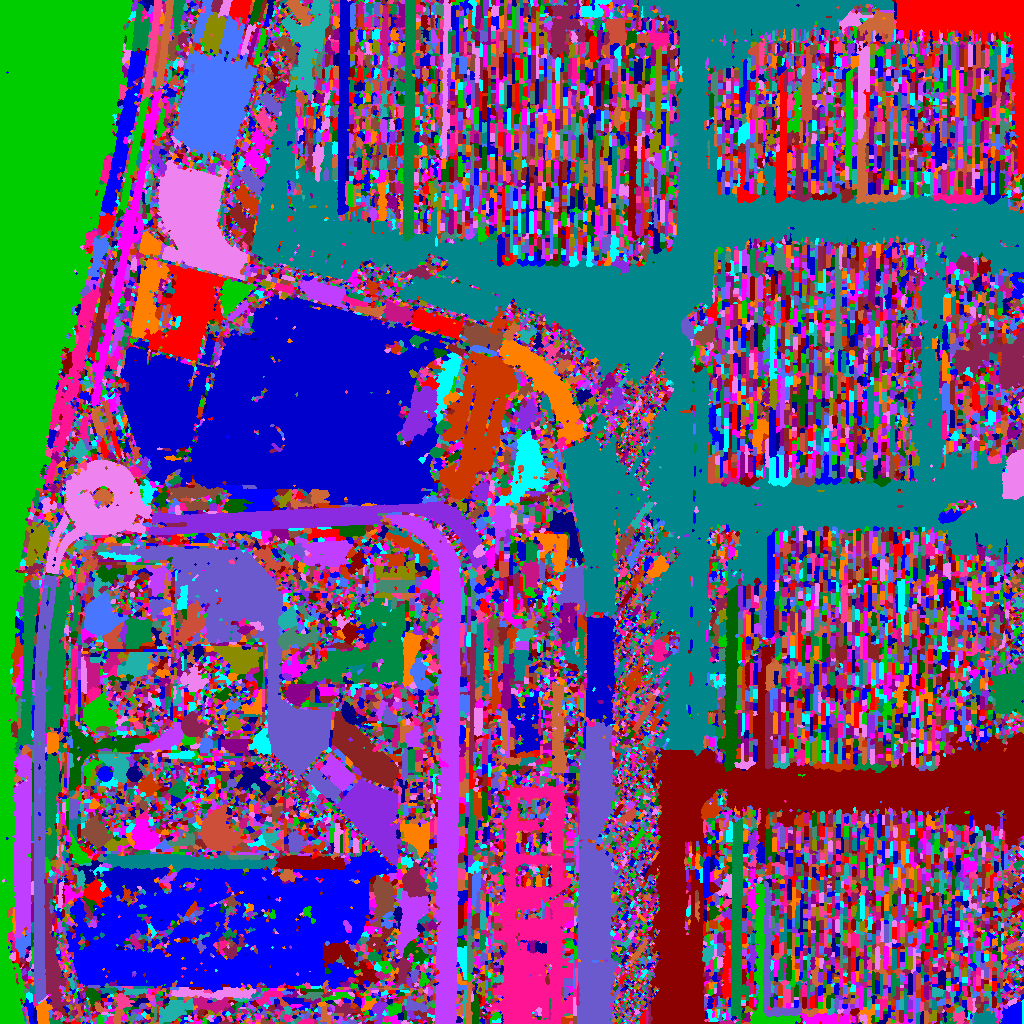
\includegraphics[width=0.3\textwidth]{Pictures/watershed_color_optimal}}
\quad
\subfigure[Mean-shift]{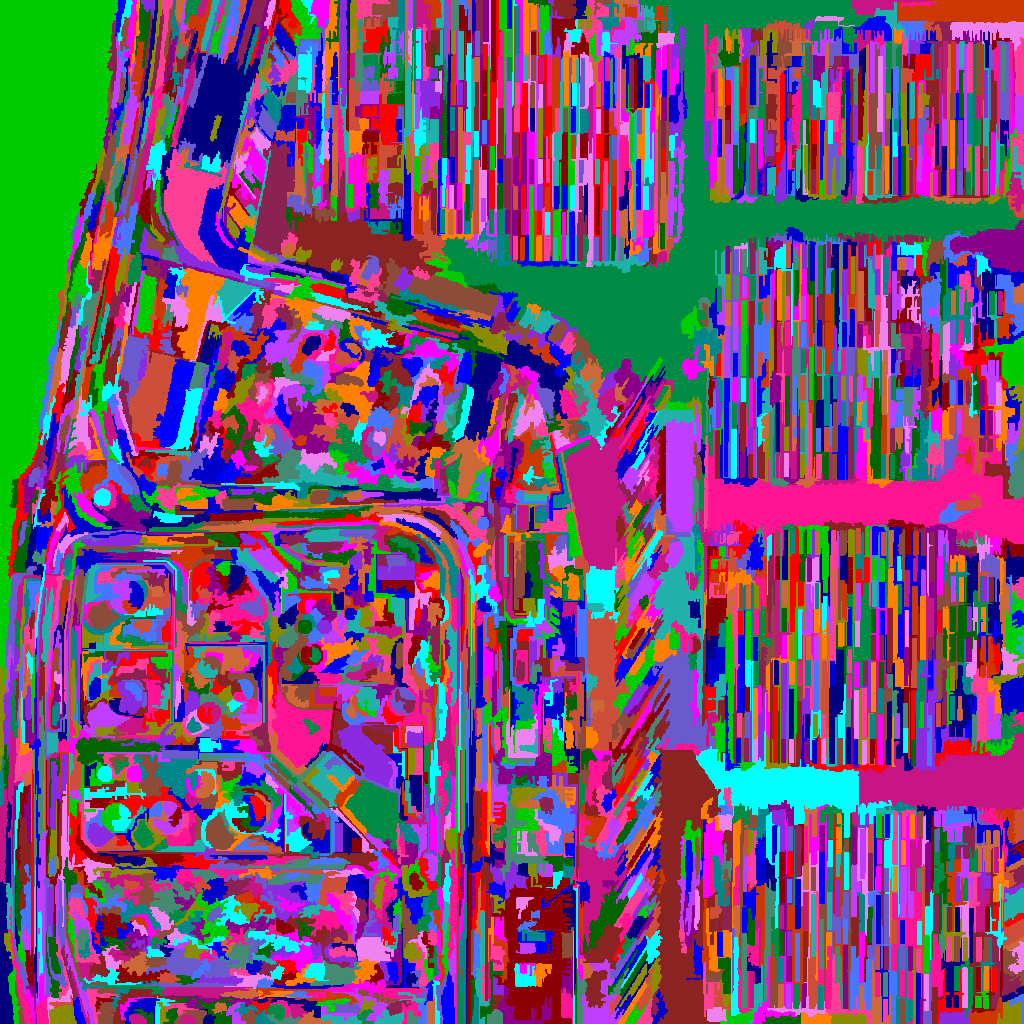
\includegraphics[width=0.3\textwidth]{Pictures/meanshift_color_optimal}}
\quad
\subfigure[Morphological Profiles]{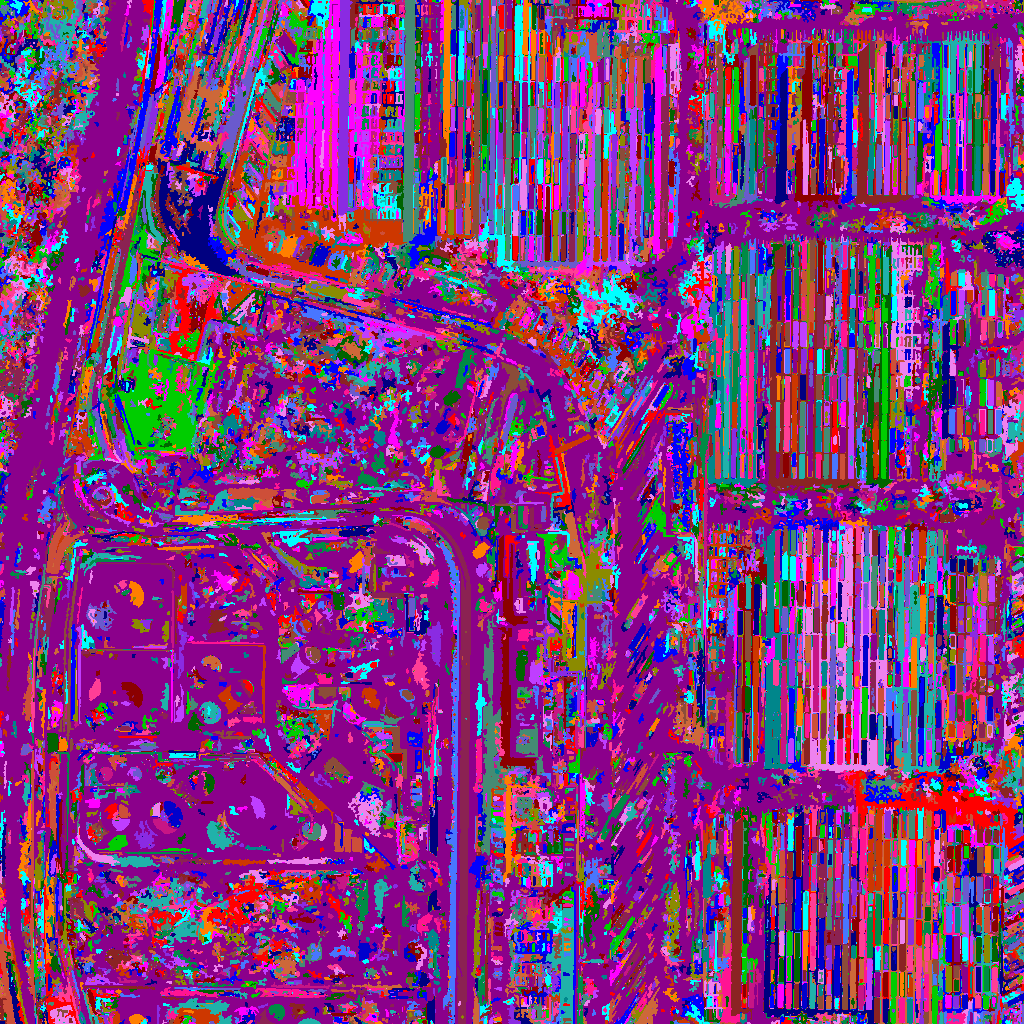
\includegraphics[width=0.3\textwidth]{Pictures/geomorpho_color_optimal}}\\

\subfigure[Watershed]{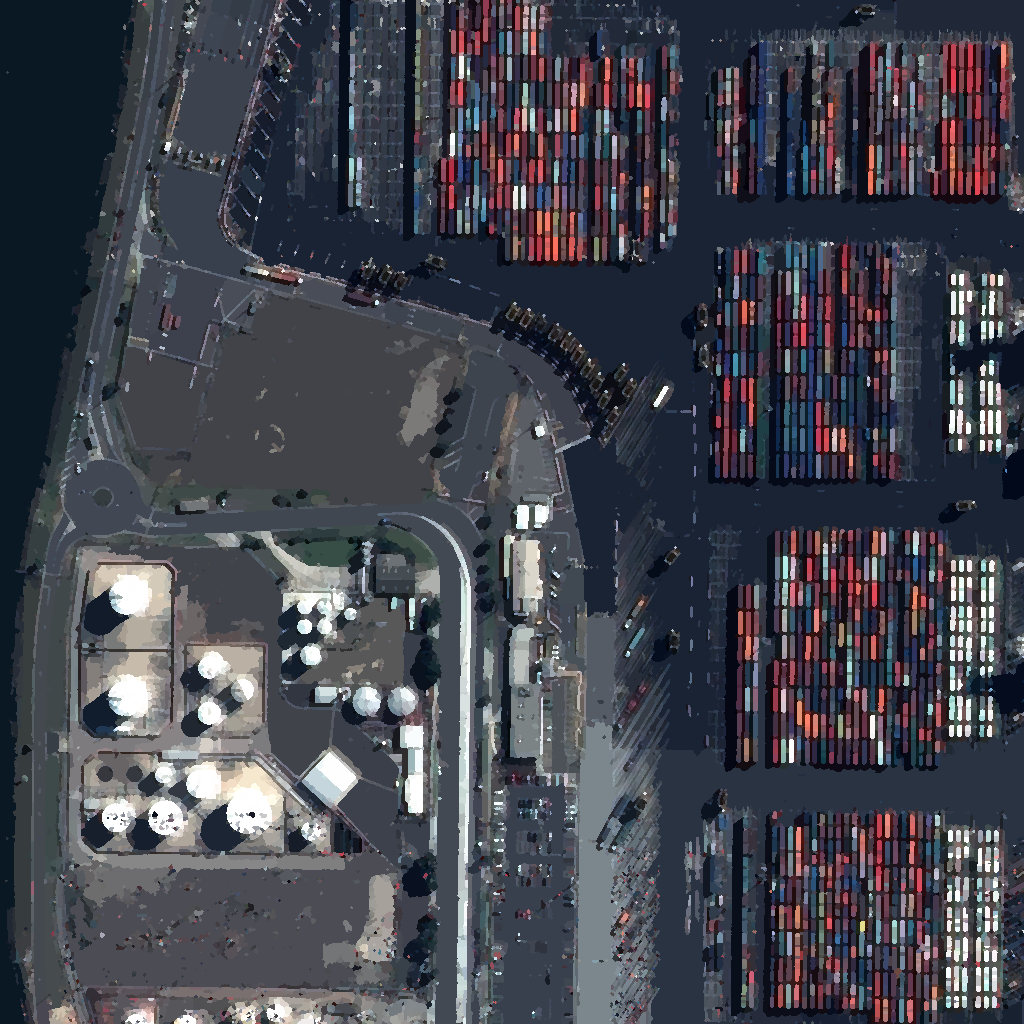
\includegraphics[width=0.3\textwidth]{Pictures/watershed_color_image}}
\quad
\subfigure[Mean-shift]{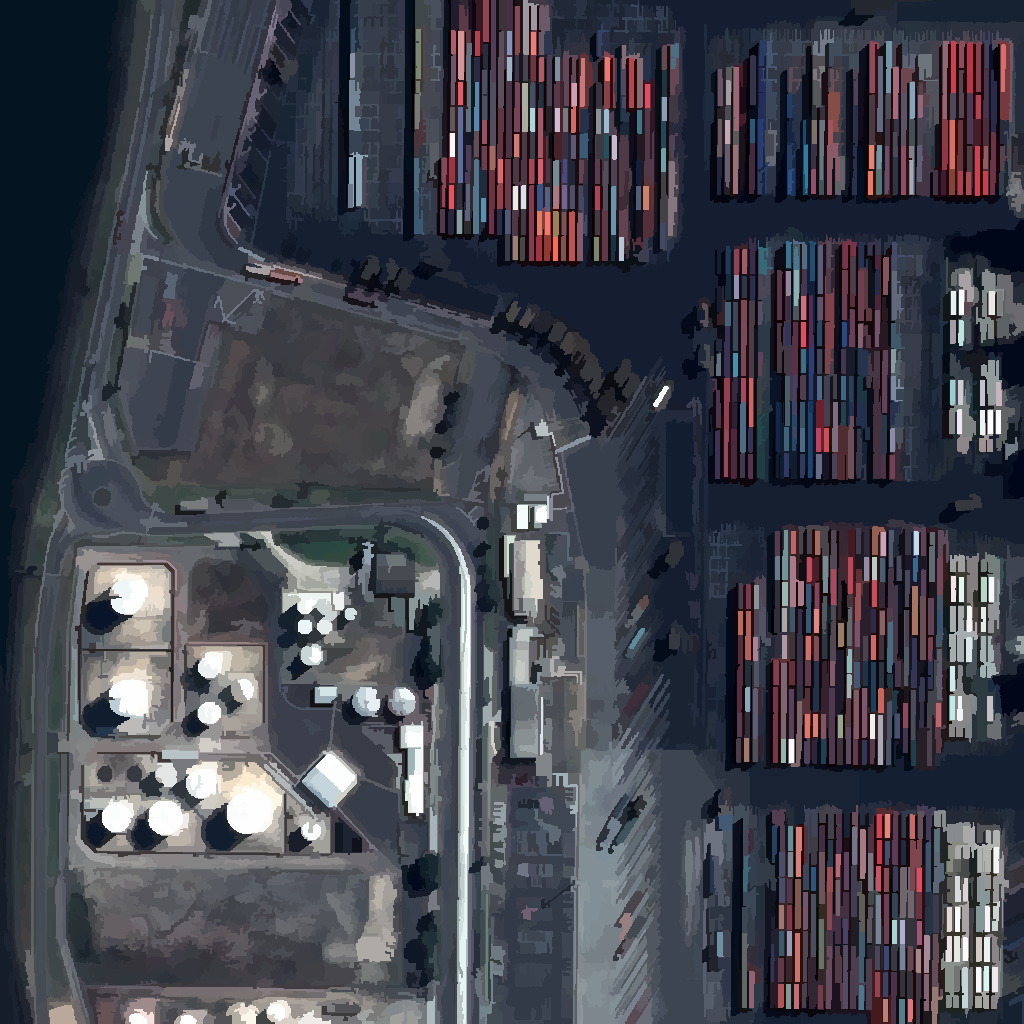
\includegraphics[width=0.3\textwidth]{Pictures/meanshift_color_image}}
\quad
\subfigure[Morphological Profiles]{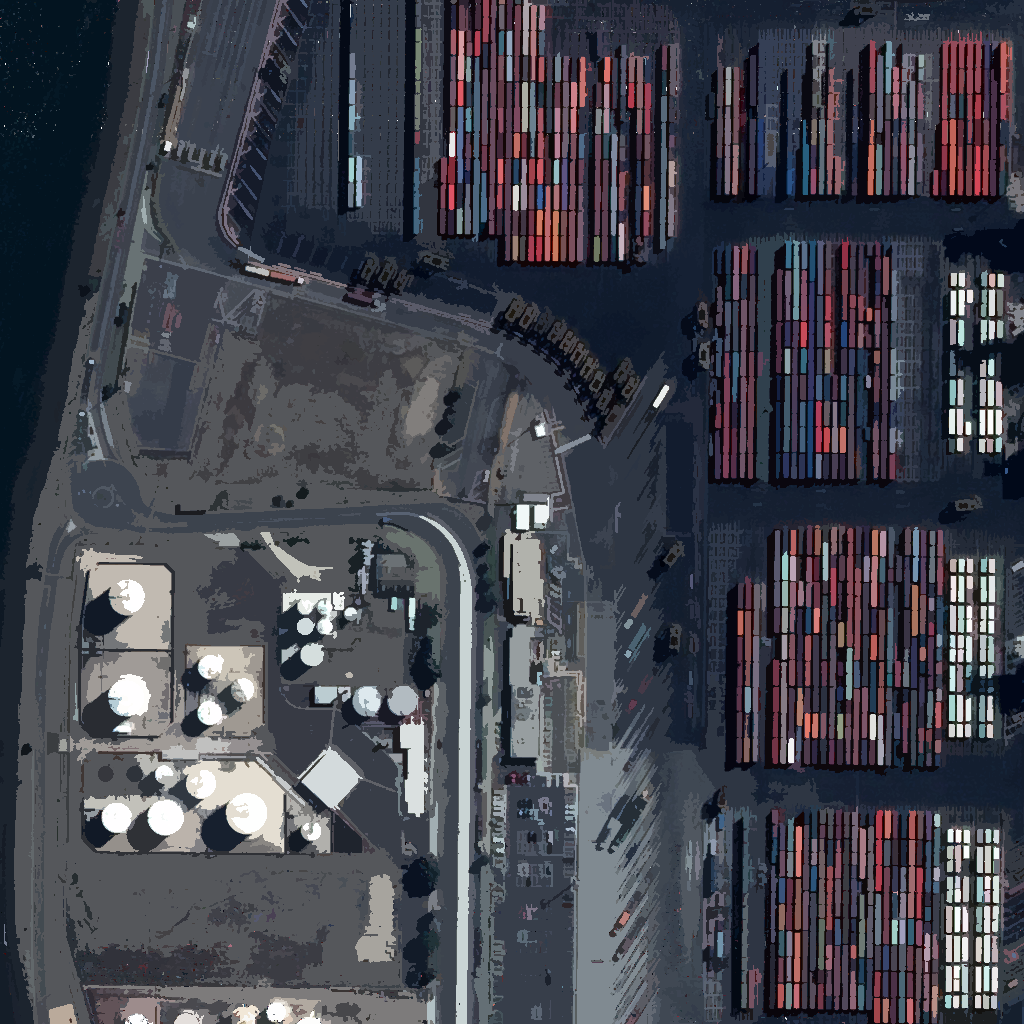
\includegraphics[width=0.3\textwidth]{Pictures/geomorpho_color_image}}
\caption{Results of various segmentation algorithms from Orfeo ToolBox
  applied on a pan-sharpened Pleiades extract. The optimal LUT (figures
  (a) to (c)) maps
  neighboring segments to highly contrasted colors, whereas the
  natural LUT (figures
  (d) to (f)) paints segment with the mean color of the underlying image.}\label{fig:segalgs}
\end{figure}


\subsection{Framework and application for large scale segmentation}

This section describes the generic framework and the segmentation
application that have been implemented in the Orfeo ToolBox. The large
scale segmentation framework works as follows:
\begin{enumerate}[1 - ]
\item Derive a tiling scheme, which depends on the following
  parameters:
\begin{itemize}
\item the amount of memory available on the computer
\item the file format of the input image (in some formats,
the image is already stored in tiles)
\item the user preferences
\end{itemize}
\item For each tile of the tiling scheme:
\begin{enumerate}[a - ]
\item Load the corresponding image part into memory
\item Segment the image extract with the segmentation algorithm
\item Polygonize the result using a filter based on GDAL capabilities,
\item Dump the polygons a file or database through OGR
      abstraction.
\end{enumerate}
\end{enumerate}

It is important to note that some tiling schemes are not suited for
this method. For instance, if the image is streamed line by line,
performing a segmentation on each line independently is irrelevant.

This framework is used in the segmentation application available in
the orfeo ToolBox, whose workflow is shown in
figure~\ref{fig:framework}. The application has two modes. The raster
mode loads the whole input image into memory and segment it with an
algorithm selected in the segmentation algorithm bank. The output is a
classical labeled raster image. The vector mode applies the large
scale segmentation framework with the selected algorithm from the
segmentation algorithms bank, and produces a vector file.

\begin{figure}[!htb]
\centering
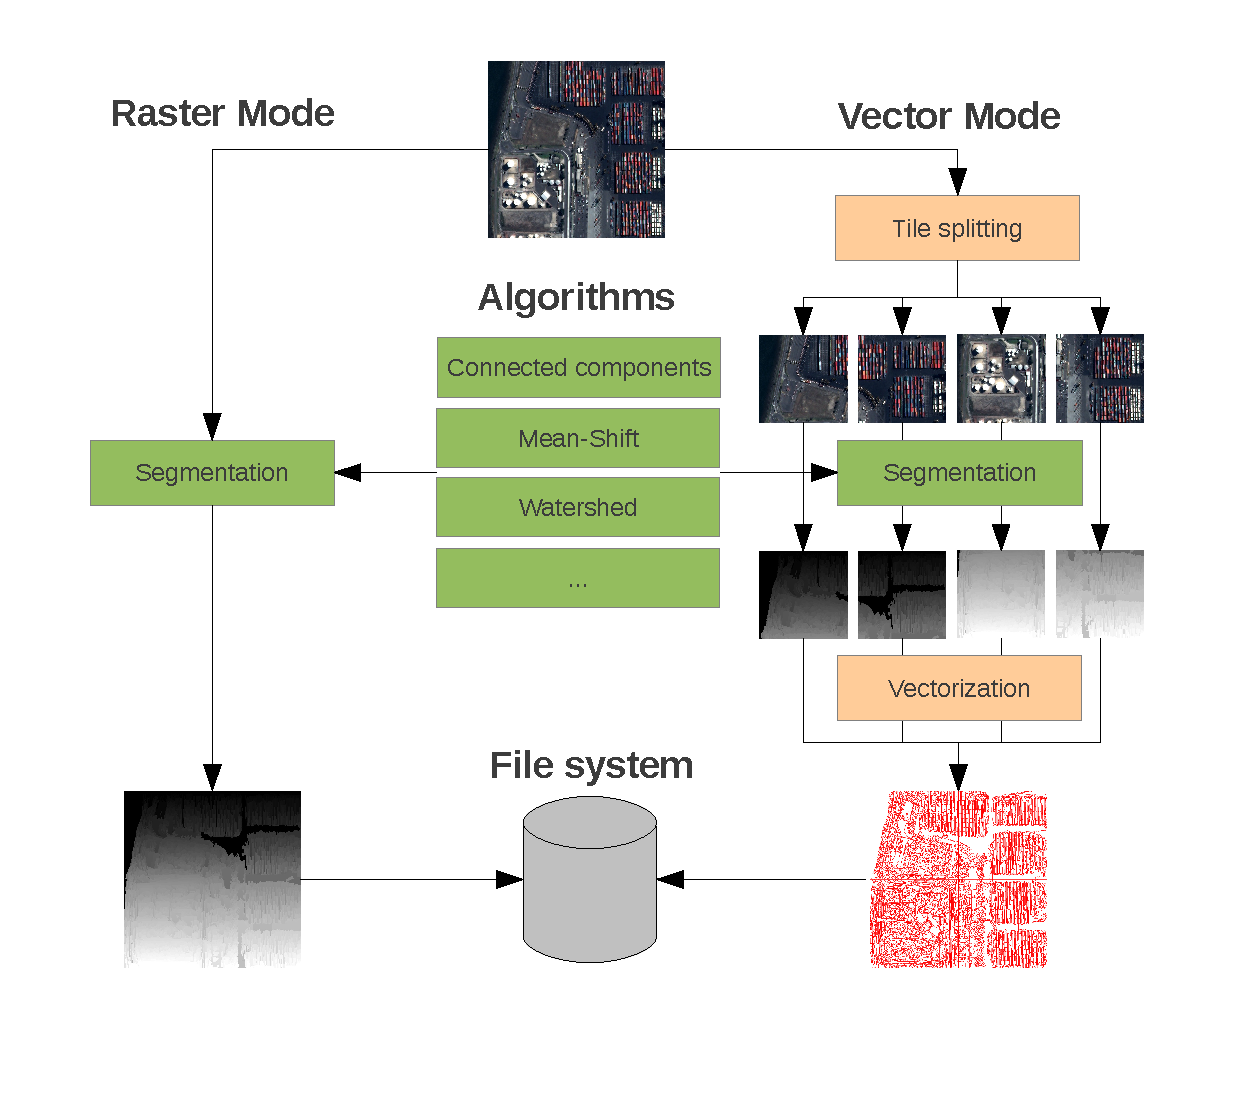
\includegraphics[width=0.8\textwidth]{Pictures/schema_ogrs}\label{fig:overview}
\caption{Overview of the large scale segmentation framework in the Orfeo ToolBox}\label{fig:framework}
\end{figure} 

The strength of this framework is that it will naturally scale up:
larger images will take more time to process and more space on file
system to store, but the system will never run out of the most limited
resource on most hardware, which is memory. The input image will still
be loaded tile by tile, and the polygons will be stored after each
tile is segmented. The most time consuming operation is the
segmentation, and this is where we allow for parallel processing
depending on the segmentation algorithm implementation. In the OTB,
the typical way to perform parallel processing is to sub-divide the
streaming tiles into smaller tiles, processed by different
threads. For instance, we implemented a multi-threaded version of the
Mean-shift algorithm~\cite{comaniciu2002mean}. This version provides a
significant performance gain when the system has multiple processor
cores.

An other key feature is that we make few assumptions on the segmentation
algorithm, so that our framework will be able to perform with any algorithms
implemented under these assumptions. Obviously, the different algorithms do not
need to share the same set of parameters. They can have their specific methods
and attributes.

Of course, this framework has the same drawbacks as other streaming
methods. Algorithms using global information in the input image will
produce different results depending on the tiling scheme, but this is
a lesser issue for segmentation algorithms that focus on local
information. The main drawback is over-segmentation : the regions
lying on tiles borders will be artificially split by the tiling
scheme. This can be a real concern when a big object that crosses
several tiles must be segmented as one region. We address these
issues in the following section.

\begin{figure}[!htb]
\centering
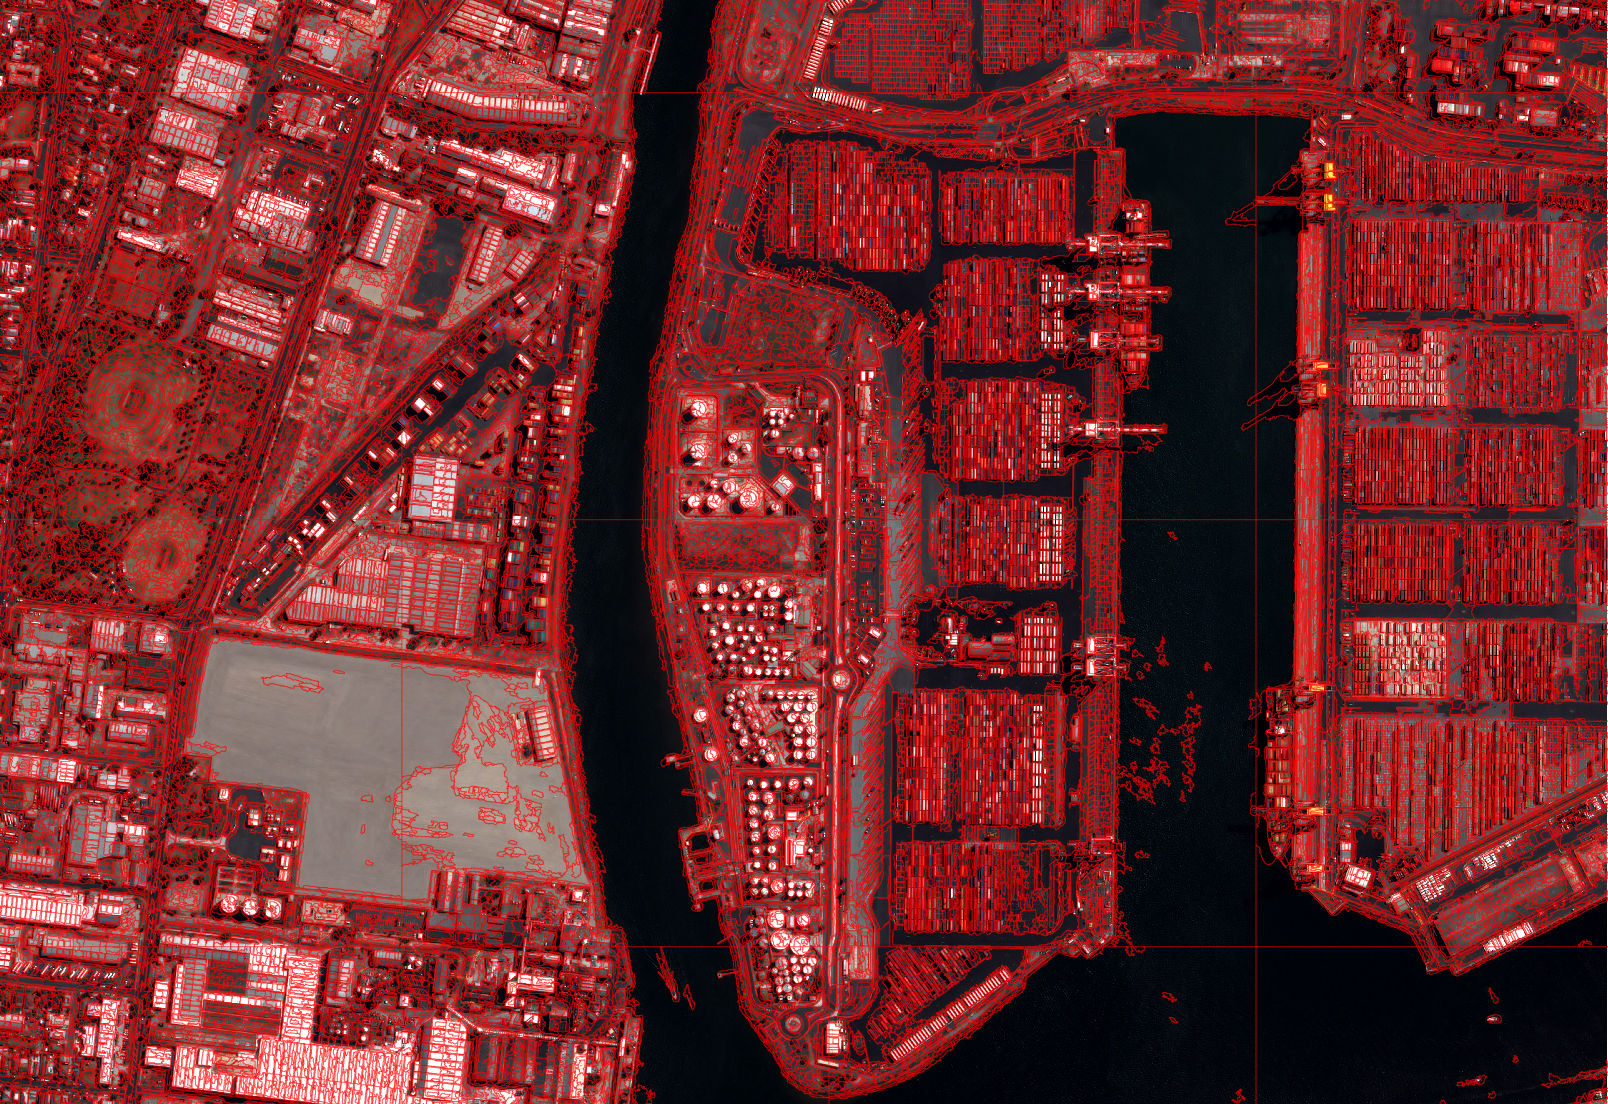
\includegraphics[width=0.9\textwidth]{Pictures/ogrs_nostitch.png}\label{fig:nostitch}
\caption{Example of large scale segmentation result from a Pleiades
  image displayed in QGIS}
\end{figure}


\subsection{Pre and post-processing to enhance usability}

In order to get useful results from this large scale segmentation, we
need to address several issues. The first one issue is the splitting
of regions on the border of tiles. The naive solution we
implemented is a simple stitching rule: we post-process the vector
data by looking for neighbor polygons lying on each side of a tile
border and merge them if their contact surface is large enough. More
sophisticated techniques might be derived in the future.

\begin{figure}[!htb]
\centering
\subfigure[Stitching overview]{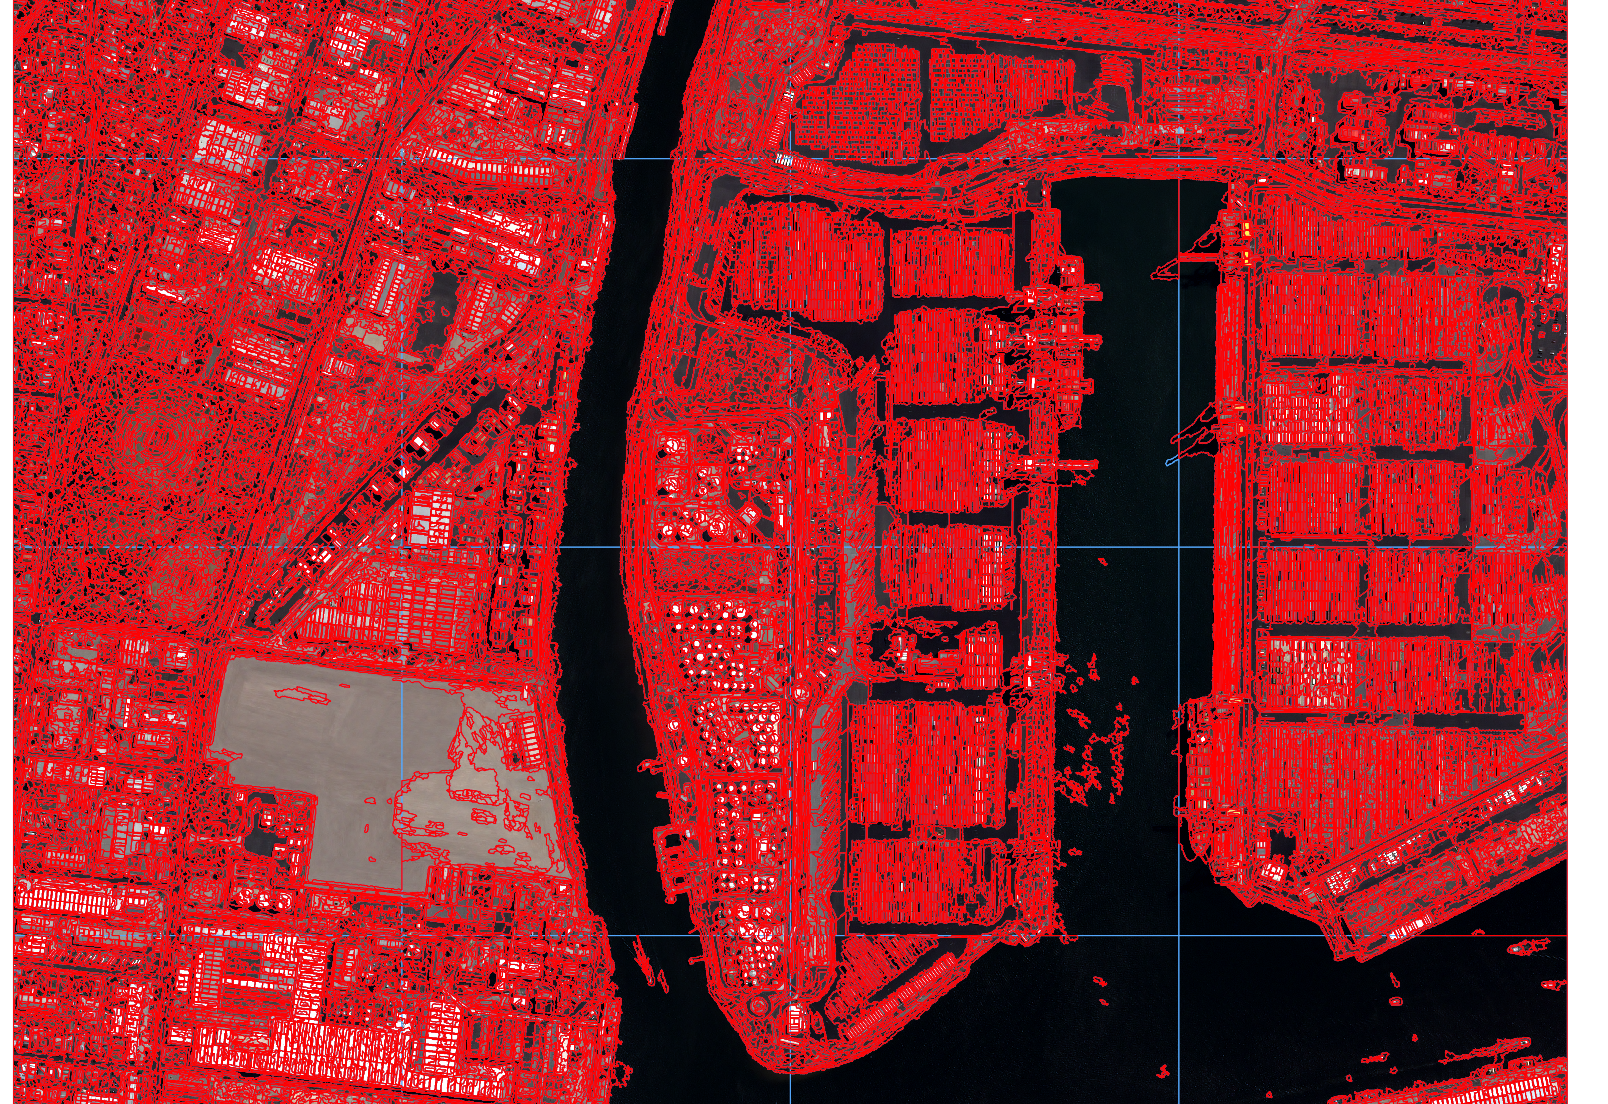
\includegraphics[width=0.9\textwidth]{Pictures/ogrs_stitch.png}\label{fig:stitch}}\\
\subfigure[Stitching off (detail)]{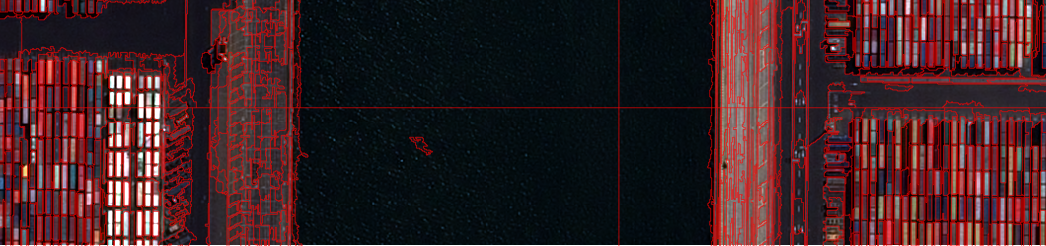
\includegraphics[width=0.45\textwidth]{Pictures/ogrs_nostitch_xt.png}}
\subfigure[Stitching on (detail)]{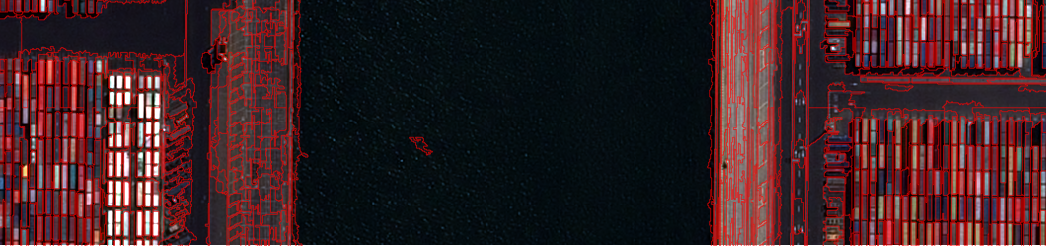
\includegraphics[width=0.45\textwidth]{Pictures/ogrs_stitch_xt.png}}
\caption{Example of large scale segmentation result from a Pleiades
  image displayed in QGIS, with stitching. Tile borders that have
  successfully been removed are displayed in blue.}
\end{figure}

The second problem is that polygons reflect exactly the shape of
the segment, and contain a large amount of vertices. This leads to
very heavy vector files, sometimes even heavier than the corresponding
raster image would be. To deal with this issue, we added
pre-processing as well as post-processing. Firstly, we added an input
mask image to avoid segmenting unwanted regions, like no-data pixels,
clouds, or vegetation (if vegetation is not desired). We also added a
rule to remove very small segments, which are more likely to
correspond to segmentation noise than to real objects (this leads to
holes in the segmentation canvas). Last, we again used the
capabilities of OGR to perform a geometry simplification algorithm,
which simplify polygons by removing vertices according to a given
tolerance.

These additional processing allows to produce a cleaner (and lighter) vector
segmentation output which can then be used in a GIS software.

\section{Conclusion}

The proposed methodology address the problem of the segmentation algorithms
scalability and allows to process full very high resolution remote sensing
images in an efficent and generic way.

This framework is only a first step toward providing an open source
large scale OBIA and spatial reasoning framework. Future developments
will include more stitching and tiling strategies to enhance the
segmentation performance at tiles borders, using approaches such as
presented in~\cite{crisp2003fast}, and the computation of attributes
along with polygons, such as statistics on radiometry from an image,
or shape attributes. These attributes could then be used for reasoning
or classification at the object level. While there is still a lot
missing, we hope to provide a comprehensive environment for
object-based techniques for VHR images analysis through the ongoing
efforts to integrate Orfeo ToolBox within Quantum
GIS\furl{www.qgis.org} \textit{via}
Sextante\furl{http://www.sextantegis.com}, and bridge the
gap between remote sensing and GIS.

\bibliographystyle{acm}
\bibliography{refs}

\end{document}
